\section{Exempelskript för viktad minsta-kvadrat anpassning}
\label{sec:matlab-wls}
Nedan finner ni ett Matlab skript ({\tt wls.m}) för viktad
minsta-kvadrat anspassning av en rät linje till en serie punkter med
uppskattad osäkerhet för varje separat punkt.

\matlabcode{matlab/wls.m}

\begin{terminaloutput}
>> wls

k =

    3.1619


m =

    2.6406


dk =

    0.2415


dm =

    1.1118
\end{terminaloutput}

Notera att vi även tog fram nya felgränser (en standardavvikelse vilket
motsvarar ett 68.27\% konfidensintervall) på våra två
parametrar. \cref{fig:matlab-wls} visar den genererade plotten.

\begin{figure}
  \centering
  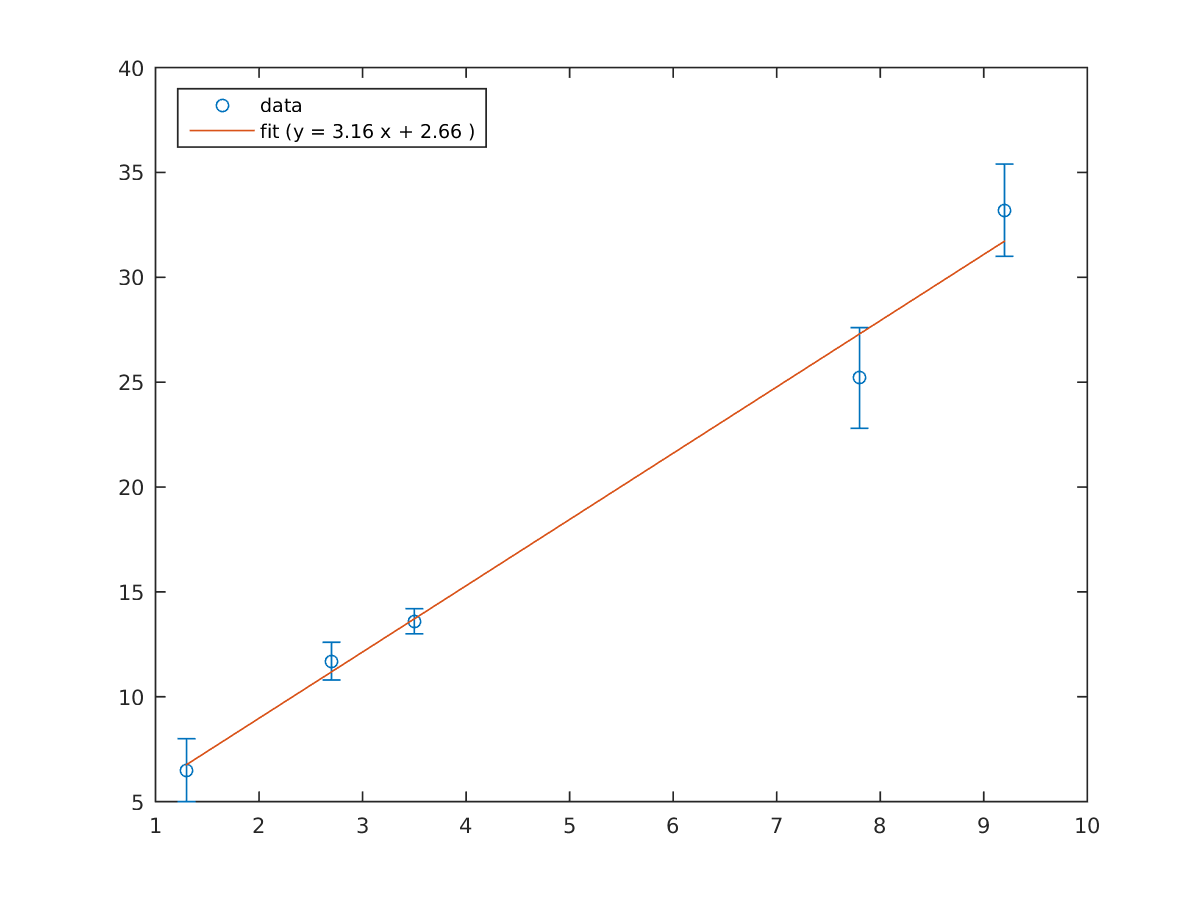
\includegraphics[scale=0.5]{matlab/wls_fit.png}
  \caption{Viktad minsta-kvadrat anpassning}
  \label{fig:matlab-wls}
\end{figure}

%%% Local Variables:
%%% mode: latex
%%% TeX-master: "../main"
%%% ispell-local-dictionary: "swedish"
%%% End:
